% !TeX root = ./proposta-pytorch.tex
\begin{titlepage}
    \clearpage\thispagestyle{empty}
	\centering

	\begin{figure}[ht]
		\centering
		
\includegraphics[height=1.25cm]{logoICMC.png}
	\end{figure}
	
	{\normalsize Universidade de São Paulo -- USP \\
		Instituto de Ciências Matemáticas e de Computação -- ICMC
		\par}
	\vspace*{2cm}
	
	{\Large\bfseries Proposta de Projeto -- AEX\par}
	\vspace*{8mm}
	{\Huge\bfseries Verão de Aprendizado Profundo \par}
	\vspace*{2mm}
	{\LARGE\bfseries \texttt{PyTorch} \emph{do Zero ao Profissional} \par}
	\vspace*{5mm}
	
    \begin{figure}[h!]
        \centering
        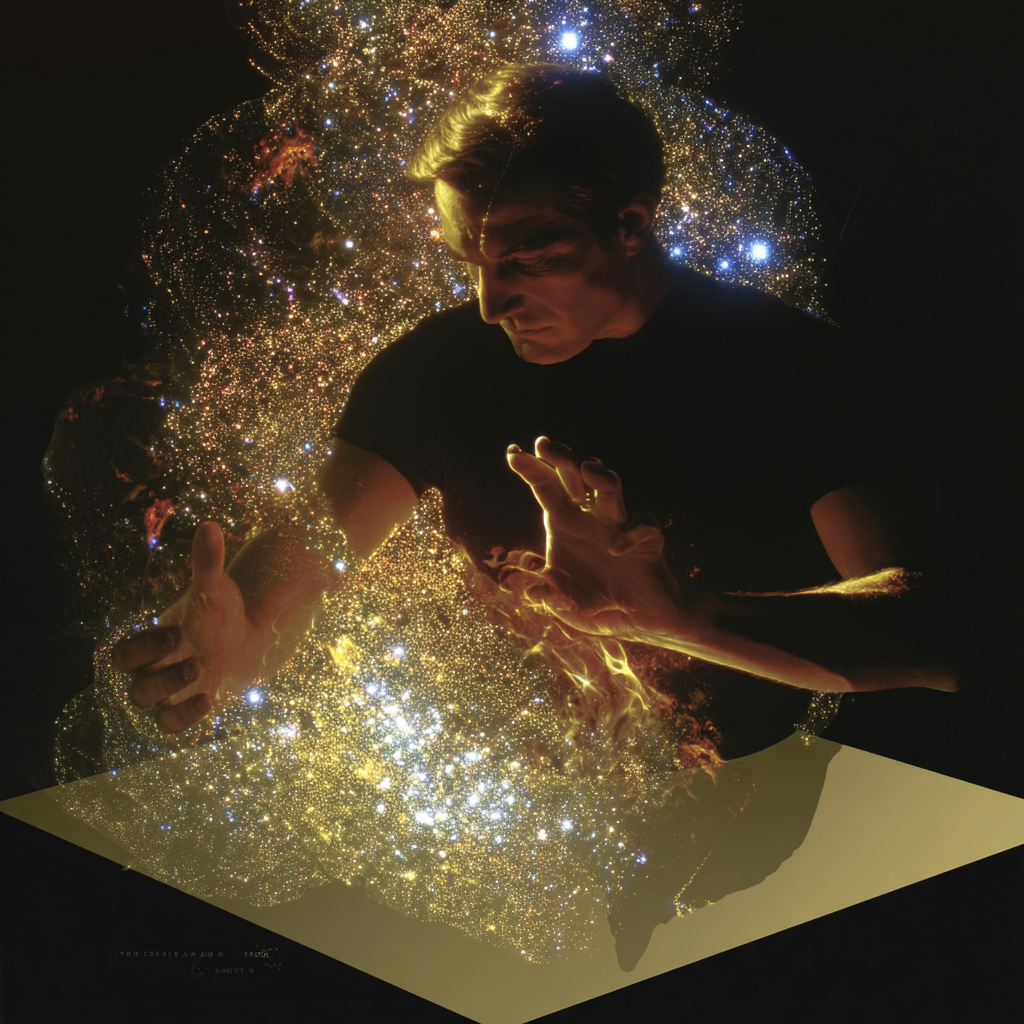
\includegraphics[width=7cm]{imagem-de-capa.png}
    \end{figure}
	\vspace*{5mm}

	\begin{tabular}{rr}
        Docente Responsável: & Prof. Dr. Lucas P. Valem \\
        Discentes: & Amanda Araujo S. \\
		& Cody S. B. Setti \\
		& Ian H. C. Bezerra
	\end{tabular}
	\vspace*{1.25cm}
	   
	\vfill  % Empurra o conteúdo restante para o final da página

	{\normalsize \today \par}
	\vspace*{2mm}
	{\normalsize São Carlos, SP, Brasil \par}
	\vspace*{2.5cm}
\end{titlepage}
